\icode{N24S-MP-SI-L2-261004-006}
\nceeID[4]{2024江苏}{5}
在原子跃迁中，辐射如图所示的4种光子，其中只有一种光子可使某金属发生光电效应，是哪一种\paren[C]

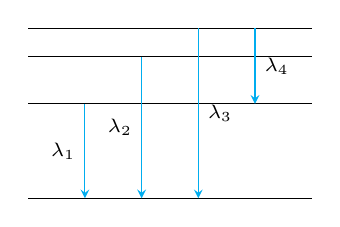
\begin{tikzpicture}[scale=1.2,font=\scriptsize,>=stealth]
	\foreach \y in {0,1,1.5,1.8}
		\draw (0,\y)--(3,\y);
	\draw[->,cyan] (.6,1)--node[left,black]{\(\lambda_1\)}(.6,0);
	\draw[->,cyan] (1.2,1.5)--node[left,black]{\(\lambda_2\)}(1.2,0);
	\draw[->,cyan] (1.8,1.8)--node[right,black]{\(\lambda_3\)}(1.8,0);
	\draw[->,cyan] (2.4,1.8)--node[right,black]{\(\lambda_4\)}(2.4,1);
\end{tikzpicture}
\begin{choices}
	\item \(\lambda_1\)
	\item \(\lambda_2\)
	\item \(\lambda_3\)
	\item \(\lambda_4\)
\end{choices}
\begin{answer}
	C\qquad 提示：\(\lambda_3\)能量最大
\end{answer}